\documentclass{article}

%% Page Margins %%
\usepackage{geometry}
\geometry{
    top = 0.75in,
    bottom = 0.75in,
    right = 0.75in,
    left = 0.75in,
}

\usepackage{amsmath}
\usepackage{graphicx}
\usepackage{parskip}

\title{Lab 4: Synchronous Sequential Circuits}

% TODO: Enter your name
\author{Frederick Meneses}

\begin{document}
\maketitle

\section*{Part I}

\begin{enumerate}
\setcounter{enumi}{1}
\item Export the subcircuit schematic as an image and include it in your report.

\begin{figure}[ht!]
    \centering
    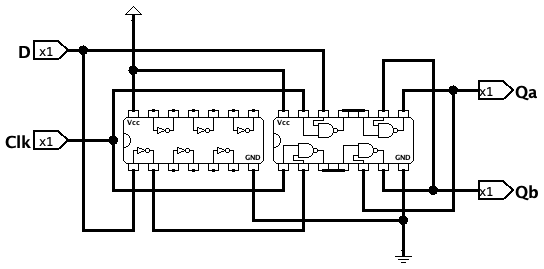
\includegraphics[width=0.5\textwidth]{lab4_gated D-latch.png}
    \caption{A schematic of the gated D-latch.}
    \label{gateddlatch}
\end{figure}


\begin{figure}[ht!]
    \centering
    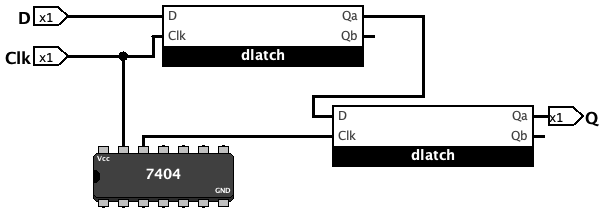
\includegraphics[width=0.5\textwidth]{lab4_D flip flop.png}
    \caption{A schematic of the D flip-flop.}
    \label{dflipdlop}
\end{figure}


\item For the D latch and the flip flop, are there any input combinations of Clk and D that should NOT be the first you test with the \emph{Poke} tool? List them if applicable.
\begin{itemize}
	\item D = 0, Clk = 0
	\item D = 1, Clk = 1
\end{itemize}
\end{enumerate}
\section*{Part IIa}

\begin{enumerate}
\setcounter{enumi}{1}
\item Export the subcircuit schematic as an image and include it in your report.

\begin{figure}[ht!]
    \centering
    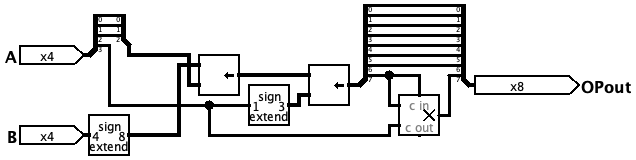
\includegraphics[width=0.4\textwidth]{lab4_op5.png}
    \caption{A schematic of op5.}
    \label{f:op5}
\end{figure}

\begin{figure}[ht!]
    \centering
    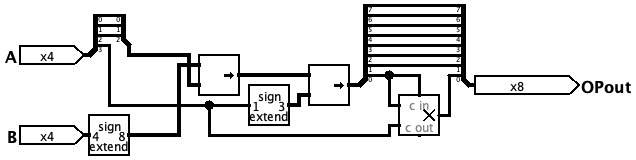
\includegraphics[width=0.4\textwidth]{lab4_op6.png}
    \caption{A schematic of op6.}
    \label{f:op6}
\end{figure}

\begin{figure}[ht!]
    \centering
    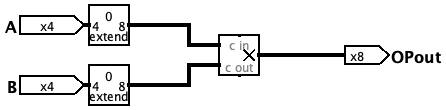
\includegraphics[width=0.4\textwidth]{lab4_op7.png}
    \caption{A schematic of op7.}
    \label{f:op7}
\end{figure}

\item Include a screenshot of your simulated test vectors for op5, op6, and op7.

\begin{figure}[ht!]
    \centering
    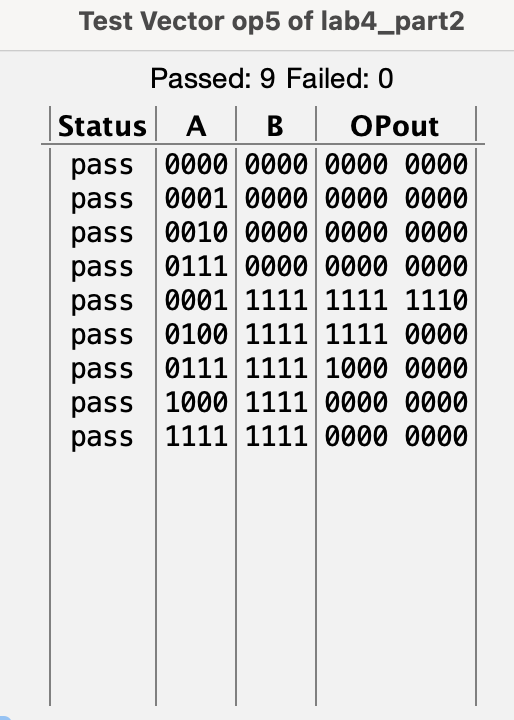
\includegraphics[width=0.4\textwidth]{lab4_op5_simulation.png}
    \caption{A simulation of op5.}
    \label{f:op5_simulation}
\end{figure}

\begin{figure}[ht!]
    \centering
    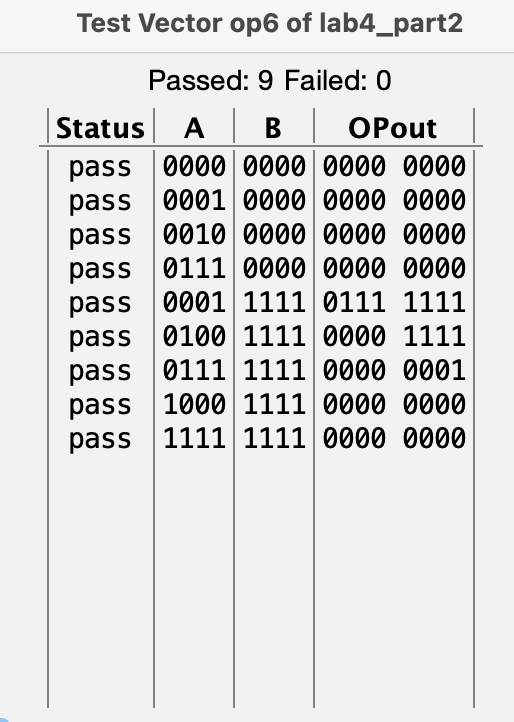
\includegraphics[width=0.4\textwidth]{lab4_op6_simulation.png}
    \caption{A simulation of op6.}
    \label{f:op6_simulation}
\end{figure}

\begin{figure}[ht!]
    \centering
    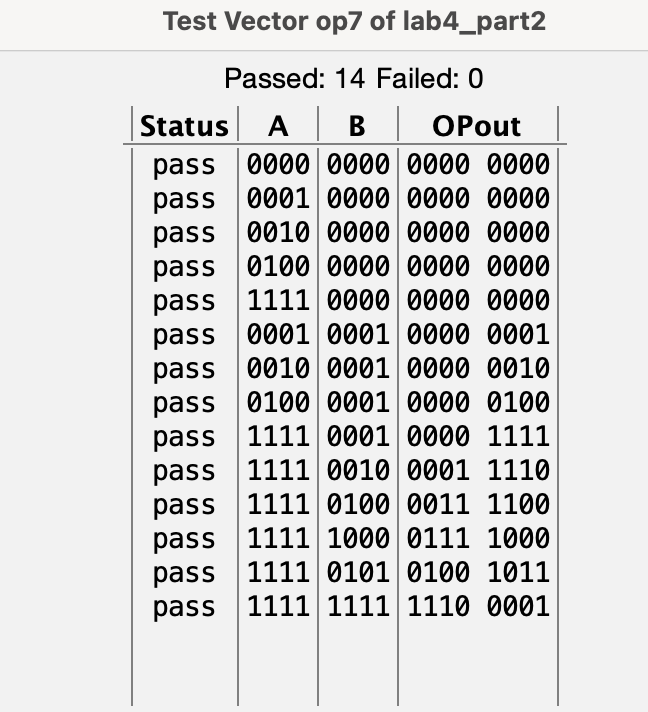
\includegraphics[width=0.4\textwidth]{lab4_op7_simulation.png}
    \caption{A simulation of op7.}
    \label{f:op7_simulation}
\end{figure}


\end{enumerate}

\section*{Part IIb}

\begin{enumerate}
\setcounter{enumi}{2}
\item Include a screenshot of your simulated timing diagram demonstrating ALUreg starting at 0x0 and increasing by 1 until 0x0f.

\begin{figure}[ht!]
    \centering
    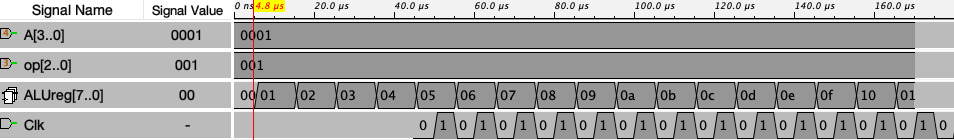
\includegraphics[width=0.5\textwidth]{lab4_timing_plus_one.png}
    \caption{A timing simulation demonstrating incrementing.}
    \label{f:timing_plus_one}
\end{figure}

\item Include a screenshot of your simulated timing diagram demonstrating a shifting operation where ALUreg goes from at 0x01 and doubling until 0x00.

\begin{figure}[ht!]
    \centering
    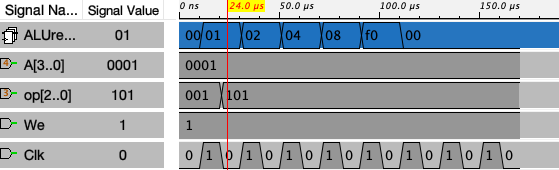
\includegraphics[width=0.4\textwidth]{lab4_timing_times_two.png}
    \caption{A timing simulation demonstrating doubling.}
    \label{f:timing_double}
\end{figure}
\end{enumerate}
\newpage
\section*{Part III}
\begin{enumerate}
\setcounter{enumi}{1}
\item What is the behaviour of the 8-bit shift register when \textit{Load\_n = 1} and \textit{ShiftRight = 0}? Briefly explain in your prelab. 
\begin{quote}
Since \textit{Load\_n = 1}, the bits from the previous clock cycle is parallel loaded into the register. However, since \textit{ShiftRight = 0}, the flip flop in each bit is not changing it's value for the bit on it's right to load.
\item Export the subcircuit schematic as an image and include it in your report.
\end{quote}

\begin{figure}[ht!]
    \centering
    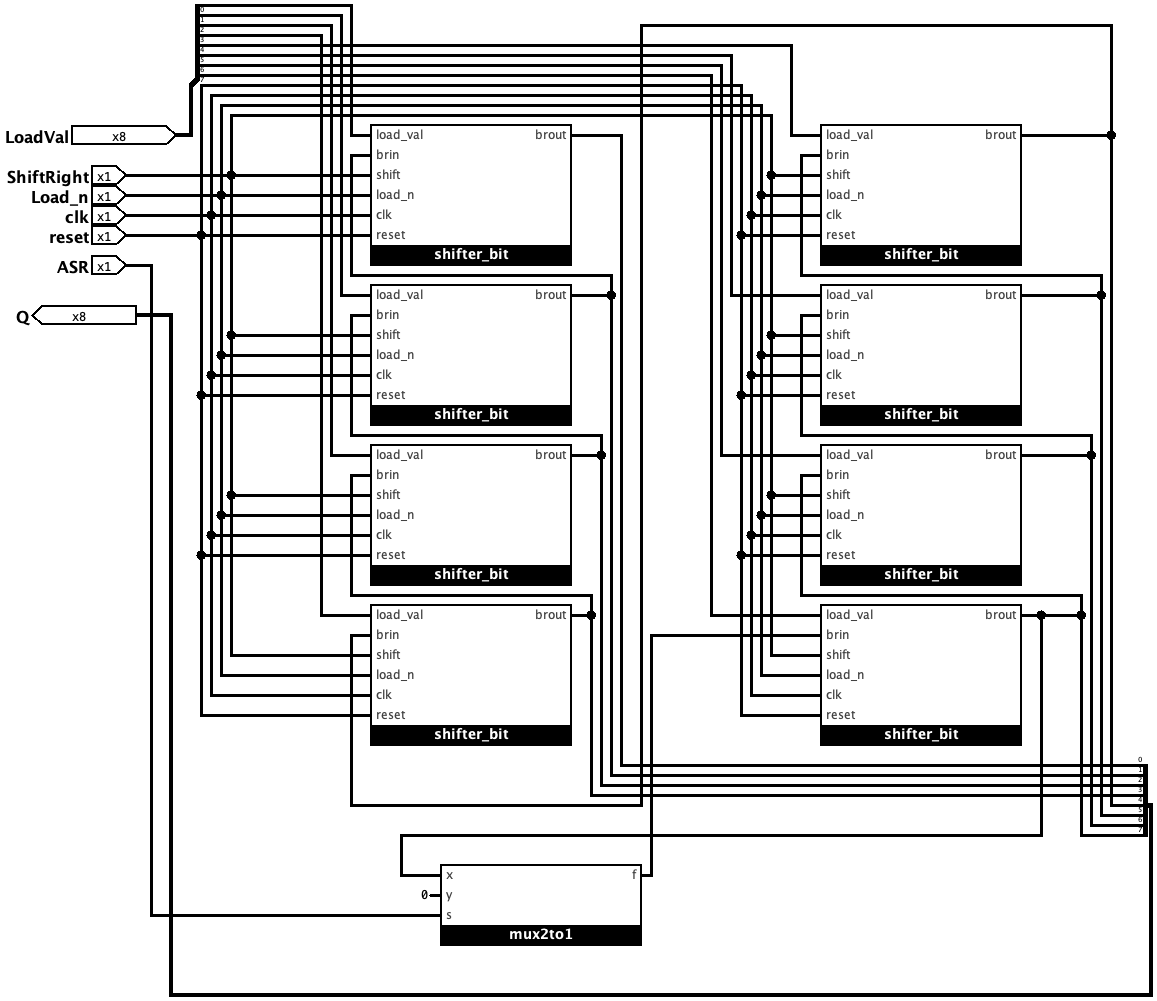
\includegraphics[width=0.5\textwidth]{lab4_shifter_bit.png}
    \caption{A schematic of the 8-bit shift register.}
    \label{f:shifter_bit}
\end{figure}

% \item Include a screenshot of your simulated timing diagram demonstrating that the output can take on values from either input.

\begin{figure}[ht!]
    \centering
    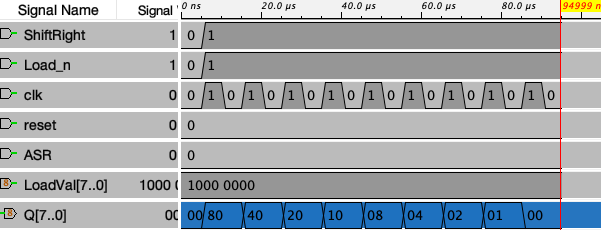
\includegraphics[width=0.5\textwidth]{lab4_timing_shift_right_one_bit.png}
    \caption{8-bit shift register's shift right one bit.}
    \label{f:timing_shifter_bit}
\end{figure}


\begin{figure}[ht!]
    \centering
    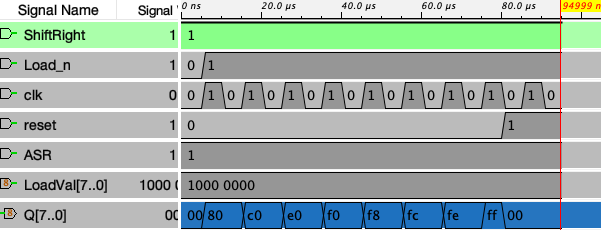
\includegraphics[width=0.5\textwidth]{lab4_timing_shift_right_asr_one_bit.png}
    \caption{8-bit shift register's shift right asr one bit with reset.}
    \label{f:timing_shifter_bit}
\end{figure}

\begin{figure}[ht!]
    \centering
    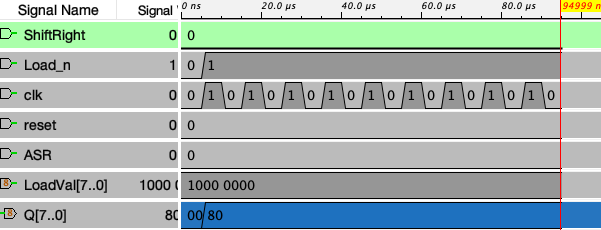
\includegraphics[width=0.5\textwidth]{lab4_timing_no_shift_load_n_one_bit.png}
    \caption{8-bit shift register's no shift load n one bit.}
    \label{f:timing_shifter_bit}
\end{figure}

\end{enumerate}

\end{document}